\subsection*{Vraag 5a}
QR en gelijktijdige iteratie berekenen alle eigenwaarden en bijhorende eigenvectoren. Gelijktijdige iteratie bij een vierkante matrix met Q(0) = I is hetzelfde als het QR algoritme zonder shift. Beide algoritme convergeren lineair.\\ [12pt]

Het QR algoritme met (RQ) shift gebruikt het principe van inverse iteratie. Dit berekent alle eigenwaarden. De Rayleigh Quot\"ent iteratie maakt ook gebruik van inverse iteratie en Rayleigh Quoti\"ent, om te convergeren naar de hoogste eigenwaarde. Beide laatsten convergeren kubisch naar hun eigenwaarden.\\ [12pt]

Alle algoritmes, behalve de Rayleigh Quoti\"ent iteratie, berekenen alle eigenwaarden.\\ [12pt]

\subsection*{Vraag 5b}
Het QR-algoritme met RQ shift past de Rayleigh Quoti\"ent iteratie toe op alle vectoren tegelijk. Het gelijktijdig toepassen op een hele matrix is het gelijktijdige iteratie algoritme, de Rayleigh Quoti\"ent iteratie is wat wordt toegepast op iedere vector.\\[12pt]

Wanneer naar het residu gekeken wordt zien we dat het Rayleigh Quoti\"ent in slechts drie stappen naar machine precisie convergeert. De gelijktijdige iteratie en QR zonder shift doet 35 iteratie stappen over het berekenen van alle eigenwaarden op machine nauwkeurigheid. QR met Rayleih Quoti\"ent shift convergeert even snel als het Rayleigh Quoti\"ent zelf, maar voor alle eigenwaarden.\\[12 pt]

\begin{figure}[!tbp]
  \centering
  \subfloat[Residu Rayleigh]{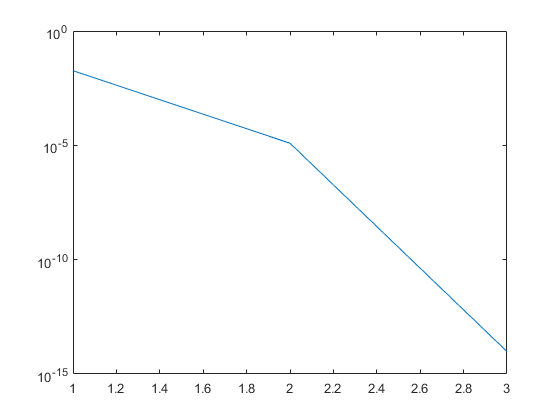
\includegraphics[width=0.5\textwidth]{Tekeningen/residu_rayleigh}\label{Residu Rayleigh}}
  \hfill
  \subfloat[Residu gelijktijdige iteratie]{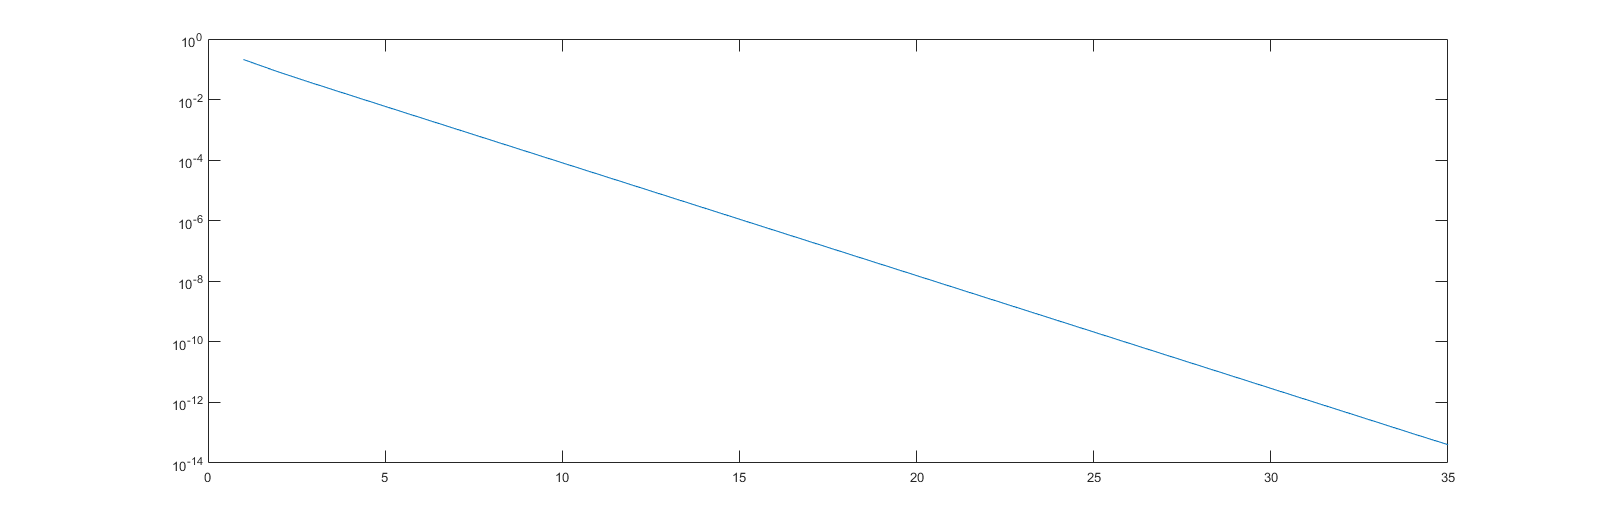
\includegraphics[width=0.5\textwidth]{Tekeningen/residu_gelijktijdige_it_randomQ}\label{Residu gelijktijdige iteratie}}
  \caption{Links residu Rayleih, rechts residu gelijktijdige iteratie.}
\end{figure}

\begin{figure}[!tbp]
  \centering
  \subfloat[Residu QR algoritme zonder shift]{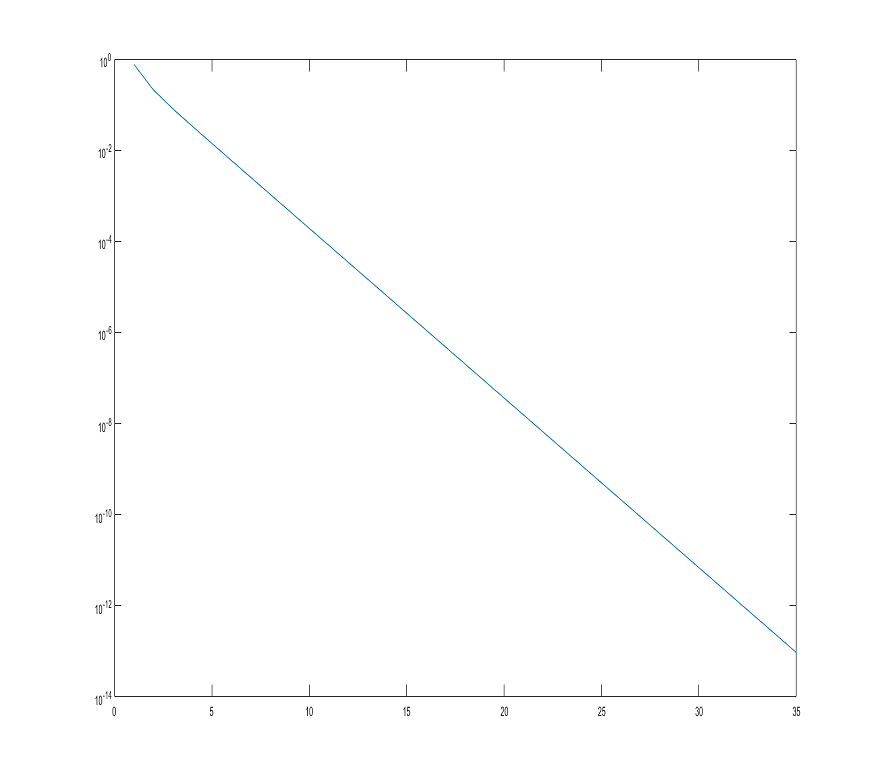
\includegraphics[width=0.5\textwidth]{Tekeningen/residu_qr_zonder}\label{Residu QR algoritme zonder shift}}
  \hfill
  \subfloat[Residu QR algoritme met Rayhleigh shift]{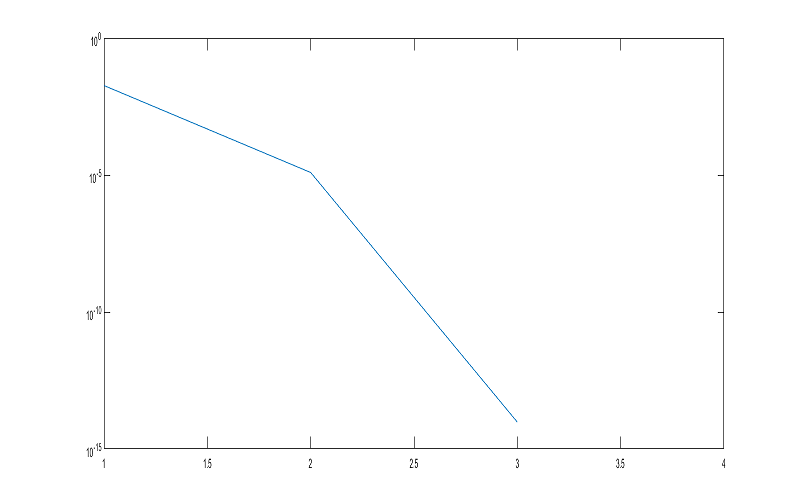
\includegraphics[width=0.5\textwidth]{Tekeningen/residu_qr_shiftrayleigh}\label{Residu QR algoritme met Rayhleigh shift}}
  \caption{Links residu QR algoritme zonder shift, rechts residu QR algoritme met Rayhleigh shift.}
\end{figure}


